\documentclass{article}

% =================================================================
%                          PACKAGES
% =================================================================

\usepackage{graphicx} % Required for inserting images
\usepackage{amsmath}
\usepackage{amssymb}
\usepackage{xcolor}
\usepackage{float}


% =================================================================
%                          TOP DOCUMENT
% =================================================================

\title{Approximation d'un problème de surface minimale}
\author{Guillaume Foucaud}
\date{Avril 2024}

% =================================================================
%                          COMMANDS AND THEOREMS
% =================================================================

\newcommand{\Integer}{ \mathbb{N} }
\newcommand{\Real}{ \mathbb{R} }
\newcommand{\Set}[1]{ \left\{ #1 \right\} }
\newcommand{\Abs}[1]{ \left| #1 \right| }
\newcommand{\Supp}[1]{\text{supp}\left( #1 \right)}

% \FunctionClass{1}{\Real}
\newcommand{\FunctionClass}[2]{ \mathcal{C}^{#1} \left( #2 \right) }

\newcommand{\FunctionClassCompact}[2]{ \mathcal{C}_c^{#1} \left( #2 \right) }

\newcommand{\FunctionWithSqrt}[1]{ \sqrt{1 + #1 ^2} }
\newcommand{\Sobolev}[1]{ W^{1,1}\left( #1 \right) }
\newcommand{\Lebesgue}[1]{ L^{1}\left( #1 \right) }
\newcommand{\Norm}[2]{ \left\| #1 \right\|_{#2} }

\newcommand{\TendsTo}[4]{#1 \xrightarrow[#2  \rightarrow #3]{} #4}

% \Integral{a}{b}{f(x)}{x}
\newcommand{\Integral}[4]{ \int_{#1}^{#2} #3 \, d#4 }

\newtheorem{question}{Question}[subsection]
\newenvironment{answer}
  {\color{blue}}
  {}

\newcommand{\QuestionAnswer}[2]{
    \begin{question}
        #1
    \end{question}
    \begin{answer}
        #2
    \end{answer}
}

\newtheorem{lemma}{Lemme}
\newtheorem{proof}{Preuve}

% document specific

\newcommand{\IntervalAB}{[a,b]}
\newcommand{\SobolevSpace}{W^{1,1}}
\newcommand{\SobolevSpaceZero}{W^{1,1}_0}
\newcommand{\HilbertSpaceZero}{H^1_0}
\newcommand{\SetC}{\mathcal{C}}
\newcommand{\FunctionJ}{\mathcal{J}}

% =================================================================
%                          DOCUMENT
% =================================================================
\begin{document}

\maketitle

Ce projet concerne l’étude d’un problème de surface minimale et
son approximation par une méthode d’élements-finis. Il comprend deux parties : la
première concerne l’étude théorique du problème. La deuxième concerne son approximation
par une méthode de descente de gradient dont l’approximation numérique
utilise la méthode des éléments-finis.
Le projet est à rendre sous la forme d’un compte rendu au format pdf. Le compte
rendu doit contenir les réponses aux questions théoriques ainsi que les résultats numériques.
Il est à envoyer à l’adresse suivante : mehdi.badsi@univ-nantes.fr. La date
limite est le mercredi 2 Mai 2024.

% = = = = = = = = = = = = = = = = = = = = = = = = = = = = = = = = =
%                          SECTION 1
% = = = = = = = = = = = = = = = = = = = = = = = = = = = = = = = = =
%\newpage
\section{Partie 1 : Étude du problème}

Soit $\Omega \subset \Real^2$ un ouvert borné et régulier et $g \in \FunctionClass{1}{\partial \Omega}$ une fonction donnée. Le problème consiste à trouver une fonction $u : \Omega \rightarrow \Real$ telle que la surface de $\Real^3$ définie par

$$\mathcal{S} = \Set{(x, y, u(x, y)) \mid (x, y) \in \Omega}$$
\newline

soit d'aire minimale et coïncide au bord de $\Omega$ avec la courbe

$$\Gamma = \Set{(x, y, g(x, y)) : (x, y) \in \partial \Omega}$$

Autrement dit, le problème s'énonce ainsi :
\newline

Trouver une fonction $u \in \FunctionClass{1}{\Omega}$ qui minimise la fonctionnelle définie par,
$$
\forall v \in \FunctionClass{1}{\Omega}, \quad J(v) = \int_{\Omega} \FunctionWithSqrt{\Norm{\nabla v}{2}} \, d(x,y)
$$
sous la contrainte $u|_{\partial \Omega} = g$,

où $\nabla v = (\partial_x v, \partial_y v)^\top$ est l'opérateur gradient usuel.

% -----------------------------------------------------------------
%                          SECTION 1.1
% -----------------------------------------------------------------

\newpage
\subsection{Étude de la fonctionnelle}

On considère la couronne $\Omega := \Set{(x, y) \in \Real^2 : a^2 < x^2 + y^2 < b^2}$ où $0 < a < b$ sont fixés. On fait l'hypothèse que la surface recherchée possède une symétrie de révolution :
$$
\exists \tilde{u} \in \FunctionClass{1}{[a, b]}, \quad \forall (x, y) \in \Omega \quad u(x, y) = \tilde{u}(\sqrt{x^2 + y^2}).
$$

% question 1
\QuestionAnswer{
    Montrer que sous l'hypothèse précédente,  $J(u) = 2\pi \Integral{a}{b}{ r \FunctionWithSqrt{ \tilde{u}'(r) }}{r}$
}{

    Soit $u \in \FunctionClass{1}{\Omega}$ tel que $u$ vérifie l'hypothèse ci-dessus.
    
    Alors, on a:
    
    \begin{equation}
    J(u) = \Integral{\Omega}{}{\FunctionWithSqrt{\Norm{\nabla v}{2}}}{\omega}
    \end{equation}

    où $\nabla u = \left( \frac{\partial u}{\partial x}, \frac{\partial u}{\partial y} \right)$.

    Or, étant donné l'hypothèse sur $u$, les dérivées partielles nous donnent :

    \begin{align*}
        \frac{\partial u}{\partial x} &= \frac{x}{\sqrt{x^2+y^2}} \tilde{u}'(\sqrt{x^2+y^2}) \\
        \frac{\partial u}{\partial y} &= \frac{y}{\sqrt{x^2+y^2}} \tilde{u}'(\sqrt{x^2+y^2}) \\
    \end{align*}

    On obtient alors :

    \begin{align*}
        \Norm{\nabla u}{2} &= {\partial_x u}^2 + {\partial_y u}^2 \\
            &= \frac{x^2}{x^2+y^2} \tilde{u}'(\sqrt{x^2+y^2})^2 + 
            \frac{y^2}{x^2+y^2} \tilde{u}'(\sqrt{x^2+y^2})^2 \\
            &= \tilde{u}'(\sqrt{x^2+y^2})^2
    \end{align*}

    Par conséquent, $J(u)$ se réécrit :

    \begin{align*}
        J(u) &= \Integral{\Omega}{}{\FunctionWithSqrt{\Norm{\nabla v}{2}}}{\omega} \\
        &= \Integral{\Omega}{}{\FunctionWithSqrt{\tilde{u}'(\sqrt{x^2+y^2})}}{(x,y)}
    \end{align*}

    On va maintenant procéder à un changement de variable pour travailler en coordonnées polaires. \newline

    Soit $\varphi :
    \begin{aligned}
    \Omega &\longrightarrow [a,b] \times [0,2\pi[\\
    (x,y) &\longmapsto (r,\theta)
    \end{aligned} \quad$ 
    tel que $
    \left\{
        \begin{array}{l}
        x = r \cos\theta \\
        y = r \sin\theta
        \end{array}
    \right.$
    
    alors $\varphi$ est un $\mathcal{C}^1$-difféomorphisme et en particulier $r=\sqrt{x^2+y^2}$. On utilise cette fonction pour notre changement de variable.

    La jacobienne de $\varphi$ se calcule comme suit :

    \begin{equation*}
        \Abs{J_\varphi(r,\theta)} =
        \begin{vmatrix}
        \frac{\partial x}{\partial r} & \frac{\partial x}{\partial \theta} \\
        \frac{\partial y}{\partial r} & \frac{\partial y}{\partial \theta}
        \end{vmatrix} = 
        \begin{vmatrix}
        \cos \theta & -r \sin \theta \\
        \sin \theta & r \cos \theta
        \end{vmatrix} = r
    \end{equation*}

    Alors, on a :

    \begin{align*}
        J(u) &= \Integral{\Omega}{}{\FunctionWithSqrt{\tilde{u}'(\sqrt{x^2+y^2})}}{(x,y)} \\
        &= \Integral{[a,b]\times[0,2\pi[}{}{ \FunctionWithSqrt{\tilde{u}'(r)}\Abs{J_\varphi(r,\theta)} }{(r,\theta)} \\
        &= \Integral{[a,b]\times[0,2\pi[}{}{ r \FunctionWithSqrt{\tilde{u}'(r)} }{(r,\theta)} \\
    \end{align*}

    De plus, en appliquant Fubini positif, on obtient :

    \begin{align*}
        J(u) &= \Integral{[a,b]\times[0,2\pi[}{}{ r \FunctionWithSqrt{\tilde{u}'(r)} }{(r,\theta)} \\
        &= \Integral{a}{b}{ \Integral{0}{2\pi}{r \FunctionWithSqrt{\tilde{u}'(r)}}{\theta} }{r} \\
        &= \Integral{a}{b}{ r \FunctionWithSqrt{\tilde{u}'(r)} }{r} \Integral{0}{2\pi}{}{\theta}\\
        &= 2\pi \Integral{a}{b}{ r \FunctionWithSqrt{\tilde{u}'(r)} }{r}\\
    \end{align*}

    On obtient finalement le résultat escompté.
}

% question 2
\QuestionAnswer{
    Justifier que la fonctionnelle donnée formellement par
    
    $$\FunctionJ(v) = \Integral{a}{b}{r\FunctionWithSqrt{v'(r)}}{r}$$
    
    est bien définie pour toute fonction $v \in \Sobolev{[a, b]}$.
    
}{
    Montrer que la fonctionnelle est bien définie revient à montrer que $\Abs{\FunctionJ(v)} < \infty$ pour tout $v \in \Sobolev{[a, b]}$. \newline
    Soit $v \in \Sobolev{[a, b]}$. On va utiliser la propriété suivante :
    \begin{equation*}
        \forall a,b \in \Real \quad \sqrt{a^2+b^2} \leq \Abs{a} + \Abs{b}
    \end{equation*}
    On a alors :
    \begin{align*}
        \Abs{\FunctionJ(v)} &= \Abs{\Integral{a}{b}{r\FunctionWithSqrt{v'(r)}}{r}} \\
        &\leq \Integral{a}{b}{r\FunctionWithSqrt{v'(r)}}{r} \quad \text{ car l'intégrande est positive} \\
        &\leq \Integral{a}{b}{r ( 1 + \Abs{v'(r)})}{r} \quad \text{ en utilisant la propriété} \\
        &\leq \Integral{a}{b}{r}{r} + \Integral{a}{b}{b\Abs{v'(r)}}{r} \quad \text{ car } r < b\\
        &\leq \frac{b^2-a^2}{2} + b \Norm{v'}{L^1}\\
    \end{align*}

    Or $v' \in L^1$ puisque $v \in \Sobolev{[a, b]}$ d'où $\Abs{\FunctionJ(v)} < \infty$
}

% question 3
\QuestionAnswer{
     Montrer qu'il existe une constante $C > 0$ telle que pour tout $v \in \Sobolev{[a, b]}$,
    
    $$\FunctionJ(v) \geq C \Norm{v'}{\Lebesgue{[a,b]}}$$
}{
    Soit $r \in ]a,b[$, alors
    $$1 + v'(r)^2 \geq v'(r)^2$$

    De plus, $0 < a < r < b$, et $x \mapsto \sqrt{x}$ est croissante, donc 
    $$r \FunctionWithSqrt{v'(r)} \geq r \Abs{v'(r)} \geq a \Abs{v'(r)} $$

    Donc en intégrant, on obtient :
    $$\Integral{a}{b}{r \FunctionWithSqrt{v'(r)}}{r} \geq a \Norm{v'}{L^1}$$
    car on rappelle que $v' \in L^1$

    Autrement dit, si on pose $C = a$ :
    $$\FunctionJ(v) \geq C \Norm{v'}{\Lebesgue{[a,b]}}$$

    
}

Soit $\alpha, \beta$ deux nombres réels avec $\alpha < \beta$. Le problème revient donc à chercher $\tilde{u} \in \Sobolev{[a, b]}$ qui minimise $ \mathcal{J} $ sur le sous-ensemble
    
$$\SetC = \Set{v \in \Sobolev{[a, b]} : v(a) = \alpha, \, v(b) = \beta }$$

% question 4
\QuestionAnswer{
     Justifier que $\SetC$ est un sous ensemble convexe et fermé de  $\Sobolev{[a, b]}$.
}{
    Montrons que $\SetC$ est convexe :

    Soient $u, v \in \SetC$ et $t \in [0, 1]$.

    $$u t + v (1-t) \in \Sobolev{[a, b]}$$ puisque $\Sobolev{[a, b]}$ est un espace vectoriel.

    Vérifions les conditions de bords.

    $$(u t + v (1-t))(a) = u(a) t + v(a) (1-t) = \alpha t + \alpha (1-t) = \alpha$$

    et

    $$(u t + v (1-t))(b) = u(b) t + v(b) (1-t) = \beta t + \beta (1-t) = \beta$$

    donc $u t + v (1-t) \in \SetC$ donc $\SetC$ est convexe.
    \newline

    Montrons que $\SetC$ est un fermé de $\Sobolev{[a, b]}$ :

    Soit une suite $(v_n)_{n \in \Integer} \in \SetC^\Integer$ tel que $\TendsTo{v_n}{n}{\infty}{v \in W^{1,1}}$. L'objectif est de montrer que $v \in \SetC$.\newline

    Conditions de bords :\newline

    On a $v_n(a) = \alpha$ et $\TendsTo{v_n}{n}{\infty}{v}$, donc si $v$ est le représentant continu, alors par unicité de la limite :
    $$\TendsTo{v_n(a)}{n}{\infty}{\alpha}$$

    De même avec $b$, l'autre condition de bord.

    Aussi, on a :

    $$\TendsTo{ \Norm{v - v_n}{W^{1,1}} }{n}{\infty}{0}$$

    donc

    $$\TendsTo{ \Norm{v - v_n}{L^1} + \Norm{v' - v_n'}{L^1} }{n}{\infty}{0}$$

    dont on déduit que :

    $$\TendsTo{ \Norm{v - v_n}{L^1} }{n}{\infty}{0}$$

    Si $v$ le représentant continu, $\TendsTo{v_n}{n}{\infty}{v}$ presque partout.

    On en conclut que $v \in \SetC$. D'où $\SetC$ fermé de $W^{1,1}[a,b]$
}

% question 5
\QuestionAnswer{
    Soit $\SobolevSpaceZero[a, b] := \Set{ v \in \Sobolev{[a, b]} \, : \, v(a) = v(b) = 0}$. Montrer que sur 
    $\SobolevSpaceZero[a, b]$, la semi norme $v \in \SobolevSpaceZero[a, b] \mapsto \Abs{v}_1 = \Norm{v'}{\Lebesgue{[a,b]}}$ est une norme 
    équivalente la norme $\Sobolev{[a, b]}$. On rappelle que la norme $\SobolevSpace$ est donnée par
    
    $$\forall v \in \Sobolev{[a, b]}, \quad \Norm{v}{\Sobolev{[a,b]}} = \Norm{v}{\Lebesgue{[a,b]}} + \Norm{v'}{\Lebesgue{[a,b]}}.$$
}{
    Pour montrer l'équivalence de ces deux normes, on veut montrer qu'il existe une constante $C_1$ et une constante $C_2$ tel que $\forall u \in \SetC$

    $$\Abs{u}_1 \leq C_1 \Norm{u}{\Sobolev{[a,b]}}$$
    $$\Norm{u}{\Sobolev{[a,b]}} \leq C_2 \Abs{u}_1$$

    Soit $u \in W^{1,1}_0$

    $$\Abs{u}_1 = \Norm{u'}{L^1} \leq \Norm{u}{L^1} + \Norm{u'}{L^1} = \Norm{u}{W^{1,1}}$$

    On pose $C_1 = 1$

    On veut montrer l'autre sens.\newline

    Directement, on a:
    \begin{align*}
        \Norm{u}{\Sobolev{[a,b]}} &= \Norm{u}{L^1} + \Norm{u'}{L^1} \\
        &= \Norm{u}{L^1} + \Abs{u}_1 \\
    \end{align*}

    Il faut donc montrer qu'il existe $K$ tel que:
    $$\Norm{u}{L^1} \leq K \Abs{u}_1$$

    Et poser $C_2 = 1 + K$

    \begin{lemma}[Signe constant]
        Soit $[s,t] \subseteq [a,b]$ tel que $u$ soit de signe constant sur $[r,s]$ et tel que $u(s)=u(t)=0$.
        Alors :
        $$\Integral{s}{t}{\Abs{u(r)}}{r} \leq b\Integral{s}{t}{\Abs{u'(r)}}{r}$$
    \end{lemma}
    \begin{proof}[Signe constant]
        \begin{align*}
            \Integral{s}{t}{\Abs{u(r)}}{r} &= \Abs{\Integral{s}{t}{u(r)}{r}}\\
            &= \Abs{[r u(r)]^t_s - \Integral{s}{t}{r u'(r)}{r}}\\
            &= \Abs{ - \Integral{s}{t}{r u'(r)}{r}} \quad \text{car u s'annule aux bords}\\
            &= \Abs{ \Integral{s}{t}{r u'(r)}{r}}\\
            &\leq  \Integral{s}{t}{\Abs{r u'(r)}}{r}\\
            &\leq b \Integral{s}{t}{\Abs{u'(r)}}{r} \quad \text{ car } 0 < s \leq  r \leq  t < b\\
        \end{align*}
    \end{proof}

    Si $u$ est le représentant continu, alors on peut décomposer :
    $$u = \sum_{i} u_i$$

    où $u_i$ a comme support $[s_i, t_i]$ et $u_i$ est de signe constant sur ce support. Chaque support est disjoint des autres.

    \begin{align*}
            \Integral{a}{b}{\Abs{u(r)}}{r} &= \sum_{i} \Integral{s_i}{t_i}{\Abs{u_i(r)}}{r} \\
            &= \sum_{i} b \Integral{s_i}{t_i}{\Abs{u_i'(r)}}{r} \quad \text{en appliquant le lemme}\\
            &= b \sum_{i} \Integral{s_i}{t_i}{\Abs{u_i'(r)}}{r}\\
            &= b  \Integral{a}{b}{\Abs{\sum_{i}u_i'(r)}}{r}\\
            &= b  \Integral{a}{b}{\Abs{\left(\sum_{i}u_i \right)'(r)}}{r}\\
            &= b  \Integral{a}{b}{\Abs{u'(r)}}{r}\\
        \end{align*}

    On obtient :
    
    $$\Integral{a}{b}{\Abs{u(r)}}{r} \leq b \Integral{a}{b}{\Abs{u'(r)}}{r}$$

    C'est à dire :
    $$\Norm{u}{L^1} \leq b \Abs{u}_1$$

    On prend $K = b$ et donc $C_2 = 1 + b$. Et on peut conclure que les deux normes sont équivalentes.
}


% question 6
\QuestionAnswer{
    En déduire que la fonctionnelle $\FunctionJ$ est coercive sur $\SetC$ et montrer que les suites minimisantes de $\FunctionJ$ sur $\SetC$ sont bornées.
}{
    On montre que $\FunctionJ$ est coercive sur $\SetC$ :\newline
    D'après la question 1.1.3 
    $$\FunctionJ(v) \geq C \Norm{v'}{\Lebesgue{[a,b]}}$$

    Mais comme $\Abs{v}_1 = \Norm{v'}{\Lebesgue{[a,b]}}$, on a :
    $$\FunctionJ(v) \geq C \Abs{v}_1$$

    Or d'après la question 1.1.5, la norme $\Abs{\cdot}_1$ est équivalente à la norme $\Norm{\cdot}{\Sobolev{[a,b]}}$, donc il existe une constante $C'$ tel que :
    $$\FunctionJ(v) \geq C \Abs{v}_1 \geq C' \Norm{v}{\Sobolev{[a,b]}}$$

    Enfin, $\SetC \subseteq \Sobolev{[a,b]}$ et

    $$\TendsTo{\FunctionJ(v)}{\Norm{v}{\SobolevSpace}}{\infty}{\infty}$$
    Donc $\FunctionJ$ est coercive sur $\SetC$\newline

    On montre que les suites minimisantes de $\FunctionJ$ sur $\SetC$ sont bornées :\newline

    Soit une suite $(v_n)_{n\in\Integer} \in \SetC^\Integer$ tq $\TendsTo{\FunctionJ(v_n)}{n}{\infty}{ \underset{v \in \SetC}{\inf} \FunctionJ(v)}$

    D'après ce qui précède, pour chaque $v_n$ il existe une constante $C$ tel que 
    $$\FunctionJ(v_n) \geq C \Norm{v_n}{\Sobolev{[a,b]}}$$

    %On note $C = \underset{n \in \Integer}{\min} \,C_n$

    Par conséquent,
    %$$ \Norm{v_n}{\Sobolev{[a,b]}} \leq \frac{1}{C_n} \FunctionJ(v_n) \leq \frac{1}{C} \FunctionJ(v_n)$$
    $$ \Norm{v_n}{\Sobolev{[a,b]}} \leq \frac{1}{C} \FunctionJ(v_n)$$

    Or $\TendsTo{\FunctionJ(v_n)}{n}{\infty}{ \underset{v \in \SetC}{\inf} \FunctionJ(v)}$, donc $\exists N \forall n \geq N \quad \FunctionJ(v_n) \leq \FunctionJ(v_N)$

    On note $M := \underset{0 \leq n \leq N}{\max}\FunctionJ(v_n)$ et on a 
    $$\forall n \quad \Norm{v_n}{\Sobolev{[a,b]}} \leq \frac{M}{C}$$
    Donc la suite $(v_n)_{n\in\Integer}$ est bien bornée.
}

% question 7
\QuestionAnswer{
    Montrer que la fonctionnelle $\FunctionJ$ est strictement convexe sur $\SetC$. En déduire que si $\FunctionJ$ admet un minimum sur $\SetC$ alors il est unique.
}{
    \begin{lemma}
        Soit la fonction $F:
    \begin{aligned}
        & \Real \longrightarrow \Real \\
        & x \longmapsto \FunctionWithSqrt{x}
    \end{aligned}$\newline
    Alors $F$ est strictement convexe sur $\Real$
    \end{lemma}

    \begin{proof}[Lemme 1]
        On a $F \in \FunctionClass{1}{\Real}$, on calcule $F'$

        $$F'(x) = \frac{x}{\FunctionWithSqrt{x}} > 0, \quad \text{si} \quad x > 0$$
        De plus $F' \in \FunctionClass{1}{\Real}$, donc on peut calculer $F''$ :

        $$F''(x) = \frac{F(x) - xF'(x)}{F(x)^2} = \frac{1 + x^2 - x^2 }{F(x)^3} = \frac{1}{\FunctionWithSqrt{x}^3} > 0 \quad \forall x \in \Real$$

        D'où $F$ strictement convexe sur $\Real$.
    \end{proof}

    \begin{lemma}
        Si $u' = v'$ presque partout avec $u,v \in \SetC$, alors $u = v$ presque partout.
    \end{lemma}

    \begin{proof}[Lemme 2]
        Soient $u,v\in \SetC$ tel que $u'=v'$ presque partout.
        Alors $u - v = C$ avec $C$ une constante.
        Or on a $u(a) - v(a)=0$, donc $C = 0$ d'où $u = v$ presque partout.
    \end{proof}

    Désormais, on montre que la fonctionnelle $\FunctionJ$ est strictement convexe sur $\SetC$.\newline

    On rappelle que pour $u \in \SetC$:
    $$\FunctionJ(u) = \Integral{a}{b}{r F(u'(r))}{r}$$

    Soit $u,v \in \SetC$ et $t \in ]0, 1[$, et on suppose que $u' \neq v'$ presque partout. D'après le lemme 1, on a pour presque tout $r \in [a,b]$:
    $$t F(u'(r)) + (1-t) F(v'(r)) - F(t u'(r) + (1-t) v'(r)) \geq 0$$

    On a l'égalité si $u' = v'$ presque partout. Mais ce n'est pas le cas puisqu'on suppose le contraire et d'après le lemme 2, on a $u \neq v$ presque partout.

    Donc $$t F(u'(r)) + (1-t) F(v'(r)) - F(t u'(r) + (1-t) v'(r)) > 0$$
    En multpliant par $r$ et en intégrant, on obtient :
    $$t \FunctionJ(u) + (1-t) \FunctionJ(v) - \FunctionJ(t u + (1 - t) v) > 0$$
    Donc $\FunctionJ$ est bien strictement convexe sur $\SetC$.\newline

    On veut maintenant montrer que si $\FunctionJ$ admet un minimum sur $\SetC$, alors il est unique.

    Soient $u$ et $v$ deux minimums globaux non égaux sur $\SetC$.
    On a $\mathcal{J}(u) = \mathcal{J}(v)$.

    Or $\frac{u+v}{2}\in \SetC$ et on sait que $\FunctionJ$ est strictement convexe, d'où $$\FunctionJ \left( \frac{u+v}{2} \right) < \frac{\FunctionJ(u)+\FunctionJ(v)}{2} = \FunctionJ(u)$$
    Ce qui contredit le fait que $u$ soit un minimum global. Et donc par l'absurde, on déduit que si $u$ existe, il est unique.\newline

    
}


On admet l’existence d’un minimiseur de $\FunctionJ$ sur $\SetC$. On souhaite à présent proposer un algorithme pour calculer ce minimiseur.

% -----------------------------------------------------------------
%                          SECTION 1.2
% -----------------------------------------------------------------

\newpage
\subsection{Une méthode de descente de gradient}

% question 1
\QuestionAnswer{
    Soit $u \in \SetC$ et $\varphi \in \FunctionClassCompact{\infty}{[a, b]}$ montrer que
    $$\Integral{a}{b}{ \frac{r \Abs{\varphi'(r)}^2 }{\FunctionWithSqrt{u'(r)}} }{r} = o(\Norm{\varphi'}{L^{\infty}}) \quad \text{ lorsque } \Norm{\varphi'}{L^{\infty}} \to 0$$
}{
    On commence par estimer cette intégrale :
    $$\Integral{a}{b}{ \frac{r}{\FunctionWithSqrt{u'(r)}} }{r} \leq \Integral{a}{b}{ r }{r} = \frac{b^2-a^2}{2}$$

    car $$\frac{1}{\FunctionWithSqrt{x}} \leq 1 \quad \forall x \in \Real$$

    On remarque que $\frac{r}{\FunctionWithSqrt{u'(r)}} \geq 0 \quad \forall r \in [a,b]$.

    En utilisant l'inégalité de Holder avec la convention $1 = 1 + \frac{1}{\infty}$, on a :
    \begin{align*}
        \Integral{a}{b}{ \frac{r\Abs{\varphi'(r)}^2 }{\FunctionWithSqrt{u'(r)}} }{r}
        &\leq \Integral{a}{b}{ \frac{r}{\FunctionWithSqrt{u'(r)}} }{r} \underset{\varphi \in \FunctionClassCompact{\infty}{[a, b]}}{\sup}\Abs{\varphi'(r)}^2\\
        &\leq \frac{b^2-a^2}{2} \Norm{\varphi'}{L^\infty}^2 \\
        &< \infty
    \end{align*}

    d'où $\Integral{a}{b}{ \frac{r \Abs{\varphi'(r)}^2 }{\FunctionWithSqrt{u'(r)}} }{r} = o(\Norm{\varphi'}{L^{\infty}}) \quad \text{ lorsque } \Norm{\varphi'}{L^{\infty}} \to 0$
    
}

% question 2
\QuestionAnswer{
    Montrer que pour tout $u \in \SetC$ et tout $\varphi \in \FunctionClassCompact{\infty}{[a, b]}$ alors $u + \varphi \in \SetC$ et
    $$\FunctionJ(u + \varphi) = \FunctionJ(u) + \Integral{a}{b}{ r \frac{u'(r)\varphi'(r)}{\FunctionWithSqrt{u'(r)}} }{r} + o(\Norm{\varphi'}{L^{\infty}}).$$
}{
    On reprend la fonction $F$ de la question 1.1.7. On sait que cette fonction est $\FunctionClass{1}{\Real}$, on applique donc un développement de Taylor-Lagrange sur cette fonction.\newline

    Soit $x, \varepsilon \in \Real$, on pose $x_0 \in [0, \varepsilon [$ tel que :

    \begin{equation}
        F(x+\varepsilon) = F(x) + \varepsilon F'(x) + \frac{\varepsilon^2}{2}F''(x + x_0)
    \end{equation}

    En prenant $x = u'(r)$ et $\varepsilon = \varphi'(r)$, on a :

    \begin{align*}
        F(u'(r)+\varphi'(r)) = F(u'(r)) + \varphi'(r) F'(u'(r)) + \frac{\varphi'(r)^2}{2}F''(u'(r) + x_0)
    \end{align*}

    En multipliant par $r$, en intégrant sur $[a,b]$ et en remplaçant $F$, $F'$ et $F''$ par leur expression calculée en question 1.1.7, on obtient :
    
    \begin{align*}
        \FunctionJ(u + \varphi) = \FunctionJ(u) + \Integral{a}{b}{ r \frac{u'(r)\varphi'(r)}{\FunctionWithSqrt{u'(r)}} }{r} + 
        \Integral{a}{b}{r \frac{\varphi'(r)^2}{2} \frac{1}{\FunctionWithSqrt{(u'(r) + x_0)}^3} }{r}
    \end{align*}

    Or, 
    \begin{align*}
        \Integral{a}{b}{ \frac{r \varphi'(r)^2}{\FunctionWithSqrt{(u'(r) + x_0)}^3} }{r} \leq \Integral{a}{b}{ \frac{r \varphi'(r)^2}{\FunctionWithSqrt{u'(r)}} }{r}
    \end{align*}

    car $u'(r) + x_0 \geq u'(r)$, et 
    $$\frac{1}{\FunctionWithSqrt{u'(r)}^3} = \frac{1}{(1 + u'(r)^2)\FunctionWithSqrt{u'(r)} } \leq \frac{1}{\FunctionWithSqrt{u'(r)}}$$

    et d'après la question 2.0.1, $$\Integral{a}{b}{ \frac{r \varphi'(r)^2}{\FunctionWithSqrt{u'(r)}} }{r} = o(\Norm{\varphi'}{L^{\infty}}) \quad \text{ lorsque } \Norm{\varphi'}{L^{\infty}} \to 0$$

    On en déduit que :

    $$ \frac{1}{2}\Integral{a}{b}{ \frac{r \varphi'(r)^2}{\FunctionWithSqrt{(u'(r) + x_0)}^3} }{r} = o(\Norm{\varphi'}{L^{\infty}}) \quad \text{ lorsque } \Norm{\varphi'}{L^{\infty}} \to 0$$

    D'où finalement :

    $$\FunctionJ(u + \varphi) = \FunctionJ(u) + \Integral{a}{b}{ r \frac{u'(r)\varphi'(r)}{\FunctionWithSqrt{u'(r)}} }{r} + o(\Norm{\varphi'}{L^{\infty}}) \quad \text{ lorsque } \Norm{\varphi'}{L^{\infty}} \to 0$$
    
}

% question 3
\QuestionAnswer{
    Soit $u \in \SetC$ fixé. Montrer que l'application linéaire $d\FunctionJ(u) : W^{1,\infty}_0[a, b] \to \Real$ donnée par
    $$\forall \varphi \in W^{1,\infty}_0[a, b], \quad d\FunctionJ(u)(\varphi) = \Integral{a}{b}{ r \frac{u'(r)\varphi'(r)}{\FunctionWithSqrt{u'(r)}} }{r}$$
    est continue sur $W^{1,\infty}_0[a, b] := \Set{ v \in W^{1,\infty}[a, b] : v(a) = v(b) = 0 }$.
}{
    Puisque $d\FunctionJ(u)$ est linéaire. Il nous suffit de montrer qu'il existe $C$ une constante tel que 
    $$\forall \varphi \in W^{1,\infty}_0[a, b] \quad 
    \Abs{d\FunctionJ(u)(\varphi)} \leq C \Norm{\varphi}{W^{1,\infty}}$$

    Soit $\varphi \in W^{1,\infty}_0[a, b]$, 
    \begin{align*}
        \Abs{d\FunctionJ(u)(\varphi)} &\leq \Integral{a}{b}{ r \frac{\Abs{u'(r)\varphi'(r)}}{\FunctionWithSqrt{u'(r)}} }{r} \\
        &\leq \Integral{a}{b}{ \frac{r}{\FunctionWithSqrt{u'(r)}} }{r} \Norm{u' \varphi'}{L^\infty} \quad \text{en utilisant l'inégalité de Holder avec} \quad 1 = 1 + \frac{1}{\infty} \\
        &\leq \frac{b^2-a^2}{2} \Norm{u'\varphi'}{L^\infty} \quad \text{en utilisant la question 1} \\
        &\leq \frac{b^2-a^2}{2} \Norm{u'}{L^\infty} \Norm{\varphi'}{L^\infty} \quad \text{en utilisant l'inégalité de Holder avec} \quad \frac{1}{\infty} = \frac{1}{\infty} + \frac{1}{\infty} \\
    \end{align*}

     De plus, $\Norm{\varphi'}{L^\infty} \leq \Norm{\varphi}{L^\infty} + \Norm{\varphi'}{L^\infty} = \Norm{\varphi}{W^{1,\infty}}$. On pose $C = \frac{b^2-a^2}{2} \Norm{u'}{L^\infty}$.

     On a donc :
     $$\Abs{d\FunctionJ(u)(\varphi)} \leq C \Norm{\varphi}{W^{1,\infty}}$$
     d'où $d\FunctionJ(u)$ continue.
}

% question 4
\QuestionAnswer{
    Soit $u \in \SetC$ fixé. Montrer que l'application linéaire précédente est aussi continue 
    sur $H^1_0[a, b]$. En déduire que le problème variationnel,

    Trouver $w(u) \in H^1_0[a, b]$ telle que pour tout $\varphi \in H^1_0[a, b]$
    $$\Integral{a}{b}{ w(u)'(r) \varphi'(r) }{r}= d\FunctionJ(u)(\varphi)$$

    admet une unique solution.
}{
    Soit $\varphi \in H^1_0[a, b]$. On repart de :

    \begin{align*}
        \Abs{d\FunctionJ(u)(\varphi)} &\leq \Integral{a}{b}{ r \frac{\Abs{u'(r)\varphi'(r)}}{\FunctionWithSqrt{u'(r)}} }{r}
    \end{align*}

    Puis, on utilise cette fois l'inégalité de Holder avec $ 1 = \frac{1}{2} + \frac{1}{2}$ :
    
    \begin{align*}
        \Abs{d\FunctionJ(u)(\varphi)}^2
        &\leq \Integral{a}{b}{ \frac{ r^2 \Abs{u'(r)}^2 }{1 + u'(r)^2} }{r} \Integral{a}{b}{ \frac{\Abs{\varphi'(r)}^2 }{1 + u'(r)^2} }{r} \\
        &\leq \Integral{a}{b}{ \frac{ r^2 \Abs{u'(r)}^2 }{1 + u'(r)^2} }{r} \Integral{a}{b}{ \Abs{\varphi'(r)}^2 }{r} \quad \text{car} \quad \frac{1}{1 + x^2} \leq 1 \quad \forall x \in \Real \\
        &\leq \Integral{a}{b}{ r^2 }{r} \Integral{a}{b}{ \Abs{\varphi'(r)}^2 }{r} \quad \text{car} \quad \frac{x^2}{1 + x^2} \leq 1 \quad \forall x \in \Real \\
        &\leq \frac{b^3-a^3}{3} \Norm{\varphi'}{L^2}^2 \\
        &\leq \frac{b^3-a^3}{3} \Norm{\varphi}{H^1}^2 \quad \text{car} \quad \Norm{\varphi'}{L^2}^2 \leq \Norm{\varphi'}{L^2}^2 + \Norm{\varphi}{L^2}^2 = \Norm{\varphi}{H^1}^2
    \end{align*}

    En posant $C = \sqrt{\frac{b^3-a^3}{3}}$, on a bien que 
    $$\Abs{d\FunctionJ(u)(\varphi)} \leq C \Norm{\varphi}{H^1}$$
    et donc que $d\FunctionJ(u)$ est continu sur $H^1_0$\newline


    On veut maintenant montrer que le problème variationnel admet une unique solution.

    Soient les fonctions :
    \begin{equation*}
        \begin{aligned}
            a: & H^1_0 \times H^1_0 \longrightarrow \Real \\
            & \vartheta,\varphi \longmapsto \Integral{a}{b}{\vartheta'(r)\varphi'(r)}{r}
        \end{aligned}
    \end{equation*}
    \begin{equation*}
        \begin{aligned}
            l: & H^1_0 \longrightarrow \Real \\
            & \varphi \longmapsto d\FunctionJ(u)(\varphi) = 
            \Integral{a}{b}{ r \frac{u'(r)\varphi'(r)}{\FunctionWithSqrt{u'(r)}} }{r}
        \end{aligned}
    \end{equation*}

    On cherche à appliquer le théorème de Lax-Milgram de sorte à montrer qu'il existe un unique $\vartheta \in H^1_0$ tel que $a(\vartheta, \varphi) = l(\varphi) \quad \forall \varphi \in H^1_0$.\newline

    On a d'après l'énoncé que $l$ est linéaire et on a montré que cette fonction était continue sur $H^1_0$[a,b]. On va maintenant montrer que $a$ est une forme bilinéaire continue et coercive.\newline

    Soient $\vartheta_1, \vartheta_2, \varphi \in H^1_0$ et $\lambda \in \Real$

    \begin{align*}
        a(\vartheta_1 + \lambda \vartheta_2, \varphi) &= 
        \Integral{a}{b}{(\vartheta_1 + \lambda \vartheta_2)'(r)\varphi'(r)}{r} \\
        &= \Integral{a}{b}{\vartheta_1'(r)\varphi'(r)}{r} + \lambda \Integral{a}{b}{\vartheta_2'(r)\varphi'(r)}{r} \\ 
        &= a(\vartheta_1, \varphi) + \lambda a(\vartheta_2, \varphi)
    \end{align*}

    donc $a$ est linéaire en sa première variable et de plus $a$ est symétrique puisque $a(\vartheta,\varphi) = a(\varphi,\vartheta)$ donc $a$ est bilinéaire.\newline

    Soient $\vartheta, \varphi \in H^1_0$

    \begin{align*}
        a(\vartheta,\varphi) &= \Integral{a}{b}{\vartheta'(r)\varphi'(r)}{r} \\
        &\leq \Integral{a}{b}{\Abs{\vartheta'(r)\varphi'(r)}}{r} \\
        &\leq \Norm{\vartheta'}{L^2} \Norm{\varphi'}{L^2} \quad \text{en utilisant l'inégalité de Cauchy-Swchartz} \\
        &\leq \Norm{\vartheta}{H^1} \Norm{\varphi}{H^1} \quad \text{car} \quad \Norm{\varphi'}{L^2} \leq \Norm{\varphi}{H^1}
    \end{align*}

    donc $a$ est continue.\newline

    Soit $\varphi \in H^1_0$

    \begin{align*}
        \Abs{a(\varphi, \varphi)} &= \Integral{a}{b}{\varphi'(r)^2}{r} \quad \text{car l'intégrande est positive}\\
        &= \Norm{\varphi'}{L^2} = \Abs{\varphi}_2 \\
        &\geq C  \Norm{\varphi}{H^1} \quad \text{car les normes } \Abs{\cdot}_2 \text{ et }\Norm{\cdot}{H^1} \text{ sont équivalentes.}
    \end{align*}

    donc $a$ est coercive.\newline

    \textbf{Remarque :} Pour l'équivalence des normes $\Abs{\cdot}_2 \text{ et }\Norm{\cdot}{H^1}$ similaire aux normes de la question 1.1.5, on utilise une propriété de cours.\newline

    D'après le théorème de Lax-Milgram, il existe un unique $\vartheta \in H^1_0$ tel que $a(\vartheta, \varphi) = l(\varphi) \quad \forall \varphi \in H^1_0$.\newline

    Or puisque l'on fixe $u$ et que $\vartheta = \omega(u)$, il existe une unique solution $\omega(u) \in H^1_0$ au problème variationnel.\newline
    
        
}

On notera par la suite $w(u) = \nabla\FunctionJ(u)$. C'est le gradient de $\FunctionJ$ en $u$ pour le produit scalaire $H^1_0$. La méthode de gradient à pas constant est définie par la suite $(u^n)_{n\in\Integer}$ qui vérifie :

\begin{equation}
(G): \left\{
\begin{aligned}
    & u^0 \in \SetC, \\
    & u^{n+1} = u^n - \rho\nabla\FunctionJ(u^n), \quad \forall n \in \Integer,
\end{aligned}
\right.
\end{equation}

où $\rho > 0$ est fixé.

% question 5
\QuestionAnswer{
    Justifier que la méthode de gradient à pas constant préserve les conditions
    aux bords.
}{
    On procède par récurrence.\newline
    Puisque $u^0 \in \SetC$, on a $u^0(a) = u^0(b) = 0$.

    Maintenant supposons que pour $n$ fixé, on ait $u^n(a)=u^n(b)=0$.

    On sait que $\nabla\FunctionJ(u^n) = w(u^n) \in H^1_0[a,b]$, donc $\nabla\FunctionJ(u^n)(a) = \nabla\FunctionJ(u^n)(b) = 0$

    Et donc, en utilisant l'hypothèse de récurrence :
    \begin{align*}
        u^{n+1}(a) &= u^n(a) - \rho\nabla\FunctionJ(u^n)(a) = 0 \\
        u^{n+1}(b) &= u^n(b) - \rho\nabla\FunctionJ(u^n)(b) = 0 \\
    \end{align*}
    
    Par conséquent,
    $$\forall n \in \Integer \quad u^n(a) = u^n(b) = 0$$
    Autrement dit, la méthode préserve les conditions de bords.
}


% = = = = = = = = = = = = = = = = = = = = = = = = = = = = = = = = =
%                          SECTION 2
% = = = = = = = = = = = = = = = = = = = = = = = = = = = = = = = = =
\newpage
\section{Partie 2 : Approximation}

Soit $N \in \Integer^*$ et $h = \frac{b-a}{N+1}$. On considère un maillage uniforme de l'intervalle $[a, b]$. On définit donc les sommets $x_i = a + ih$ pour tout $i = 0, \ldots, N+1$, et on pose

$$ V_h := \Set{ v \in \FunctionClass{0}{[a, b]} : v|_{[x_i,x_{i+1}]} \in \mathbb{P}_1, \; \forall i = 0, \ldots, N } $$
$$ V_{h,0} := \Set{ v \in V_h : v(a) = v(b) = 0 }.$$

% question 1
\QuestionAnswer{
    Montrer que $V_h$ est un espace d'approximation conforme de $W^{1,1}[a, b]$ et que $V_{h,0}$ est un espace d'approximation conforme de $H^1_0[a, b]$.
}{
    Soit $v \in V_h$, alors $v \in \FunctionClass{0}{[a,b]}$, en particulier $v \in L^1[a,b]$, et de plus $v \in \FunctionClass{1}{\bigcup_{i=0}^N]x_i, x_{u+1}[}$. Donc $v'$ est continue par morceau et en particulier $v' \in L^1$. On en déduit que $v \in W^{1,1}$. D'où $V_h \subseteq W^{1,1}$, autrement dit $V_h$ est un espace conforme de $W^{1,1}$.

    Par des raisonnements analogues, on peut montrer que $V_{h,0} \subseteq H^1_0$ si de plus on vérifie que $v(a) = v(b) = 0$ ce qui est le cas pour $v \in V_{h,0}$. Donc $V_{h,0}$ est un espace d'approcimation conforme de $H^1_0[a, b]$.
}

% question 2
\QuestionAnswer{
    Rappeler la dimension de l'espace $V_h$ et l'expression des fonctions chapeaux. Quelle est la dimension de $V_{h,0}$?
}{
    
    Puisqu'il y a $N$ intervalles sur lesquels on a restreint $v \in V_h$. On en déduit que $\dim V_h = N + 2$\newline

    On rappelle que les fonctions chapeaux sont définies comme ceci :\newline

    $\forall \, 1 \leq i \leq N \quad \forall x \in [a,b]$
    \begin{equation*}
        \omega_i (x) = 
        \begin{cases} 
        \frac{x - x_{i-1}}{x_i - x_{i-1}} & \text{si } x \in [x_{i-1}, x_i] \\
        \frac{x_{i+1} - x}{x_{i+1} - x_i} & \text{si } x \in [x_i, x_{i+1}] \\
        0 & \text{sinon}
        \end{cases}
    \end{equation*}

    Puisqu'on a fixé deux conditions de bords, on a $\dim V_{h,0} = \dim V_h - 2 = N$
}

% question 3
\QuestionAnswer{
    Le problème variationnel discret associé à la méthode de gradient est défini par la suite $(u^n_h)_{n\in\Integer}$ qui vérifie :
    \begin{equation*}
    (G): \left\{
    \begin{aligned}
        & u^0_h \in \SetC, \\
        & u^{n+1}_h = u^n_h - \rho\nabla_h\mathcal{J}(u^n_h), \quad \forall n \in \Integer,
    \end{aligned}
    \right.
    \end{equation*}
    où $\nabla_h\FunctionJ(u^n_h) \in V_{h,0}$ vérifie le problème variationnel discret :
    $$\Integral{a}{b}{ \nabla_h\FunctionJ(u^n_h)(r)\varphi'(r) }{r} = d\FunctionJ(u^n_h)(\varphi), \quad \forall \varphi \in V_{h,0}.$$
    Montrer que la suite $(u^n_h)_{n\in\Integer}$ est bien définie, i.e., $u^n_h \in \SetC$ pour tout $n \in \Integer$.
}{
    Par définition de la méthode, $u^0_h \in \SetC$.

    On fixe $n \in \Integer$ et on suppose que $u^n_h \in \SetC$. On veut montrer que $u^{n+1}_h \in \SetC$ :

    D'après la question 1.2.5, la méthode préserve les conditions de bords. De plus, on sait de la question 1.2.4 que $\nabla_h\mathcal{J}(u^n_h) \in H^1_0$

    \begin{lemma}
        Soit $u \in H^1[a,b]$, alors $u \in W^{1,1}[a,b]$
    \end{lemma}
    On peut le montrer car $[a,b]$ est de mesure finie et on peut appliquer une inégalité de Cauchy Schwartz.\newline

    D'après ce lemme, $\nabla_h\mathcal{J}(u^n_h) \in W^{1,1}[a,b]$

    Or $W^{1,1}[a,b]$ est un espace vectoriel, donc pour $\rho \in \Real$ :

    $$u^n_h - \rho\nabla_h\mathcal{J}(u^n_h) \in W^{1,1}_0[a,b]$$

    d'où $u^{n+1}_h \in W^{1,1}[a,b]$, et par récurrence, pour tout $n \in \Integer \quad u^{n}_h \in W^{1,1}[a,b]$.
    Puisqu'on a préservation des conditions de bord, pour tout $n \in \Integer \quad u^{n}_h \in \SetC$.
    
}

% question 4
\QuestionAnswer{
    Écrire la forme matricielle du problème discret pour le calcul du gradient. On précisera les expressions de la matrice de rigidité et du second membre.
}{

    On se place dans $V_n \subseteq V$. On note $d_n = \dim V_n$. Les fonctions chapeaux $w_i$ forment une base de $V_n$ avec $1 \leq i \leq d_n$, par conséquent on peut écrire la solution approximée qui nous intéresse comme :
    $$u_n = \sum^{d_n}_{i=1} \lambda_i \omega_i$$
    Le problème discret peut être écrit sous la forme matricielle suivante :

    \begin{equation*}
        A_n \bar{u}_n = b_n
    \end{equation*}

    avec $\forall i, j \in [1, N]$
    \begin{align*}
        &\bar{u}_n = (\lambda_1, \dots ,\lambda_{d_n})^T \\
        &(A_n)_{i,j} = a(\omega_j, \omega_i) \\
        &(b_n)_{i} = l(\omega_i) \\
    \end{align*}

    On rappelle que :

    \begin{align*}
        & a(\omega_j, \omega_i) = \Integral{a}{b}{\omega_j'(r)\omega_i'(r)}{r} \\
        & l(\omega_i) = d\FunctionJ(u)(\omega_i) = 
            \Integral{a}{b}{ r \frac{u'(r)\omega_i'(r)}{\FunctionWithSqrt{u'(r)}} }{r} \\
    \end{align*}

    Aussi, $\omega_i$ a une dérivée faible que l'on peut écrire :
    $$\omega_i' = \frac{1}{h} 1_{[x_{i-1}, x_i]} - \frac{1}{h} 1_{[x_i, x_{i+1}]} \quad \text{donc} \quad \Abs{\omega_i'}^2 = \frac{1}{h^2} 1_{[x_{i-1}, x_{i+1}]}$$

    avec $h = x_{i+1} - x_i \quad \forall 1 \leq i \leq d_n$\newline

    Calculons la matrice de rigidité :\newline
    $A_n$ est symétrique car $a$ est bilinéaire symétrique. De plus, $\omega_j'(r)\omega_i'(r) = 0$ si $\Abs{i - j} > 1$ pour presque tout $r$, donc $(A_n)_{i,j} = 0$ si $\Abs{i - j} > 1$. Puisque $A_n$ est symétrique, il reste deux cas à calculer : la diagonale et la sous-diagonale.\newline

    Cas de la diagonale, quand $i = j$:

    \begin{align*}
        a(\omega_i, \omega_i) &= \Integral{a}{b}{ \Abs{\omega_i'(r)}^2 }{r} \\
        &= \Integral{x_{i-1}}{x_{i+1}}{ \Abs{\omega_i'(r)}^2 }{r} \\
        &= \frac{1}{h^2} \Integral{x_{i-1}}{x_{i+1}}{ 1_{[x_{i-1}, x_{i+1}]} }{r} \\
        &= \frac{1}{h^2} 2h = \frac{2}{h} \\
    \end{align*}
    
    Cas de la sous-diagonale, quand $i-1 = j$:

    \begin{align*}
        a(\omega_{i-1}, \omega_i) &= \Integral{a}{b}{ \omega_{i-1}'(r)\omega_i'(r) }{r} \\
        &= \Integral{x_{i-1}}{x_{i+1}}{ \omega_{i-1}'(r)\omega_i'(r) }{r} \\
        &= \frac{1}{h}\Integral{x_{i-1}}{x_{i}}{ \omega_{i-1}'(r) }{r} - \frac{1}{h}\Integral{x_{i}}{x_{i+1}}{ \omega_{i-1}'(r) }{r} \\
        &= \frac{1}{h}\Integral{x_{i-1}}{x_{i}}{ \omega_{i-1}'(r) }{r} \\
        &= \frac{1}{h}\Integral{x_{i-1}}{x_{i}}{ \frac{-1}{h} }{r} \\
        &= \frac{-1}{h} \quad \forall \, 2 \leq i \leq d_n\\
    \end{align*}

    Calculons le vecteur en second membre :

    \begin{align*}
        l(w_i) &= d\FunctionJ(u)(w_i) \\
        &= \Integral{a}{b}{ r \frac{u'(r)w_i'(r)}{\FunctionWithSqrt{u'(r)}} }{r} \\
        &= \Integral{x_{i-1}}{x_{i+1}}{ r \frac{u'(r)w_i'(r)}{\FunctionWithSqrt{u'(r)}} }{r} \quad \text{car } \Supp{\omega_i} = [x_{i-1},x_{i+1}] \\
        &= \frac{1}{h} \Integral{x_{i-1}}{x_{i}}{ r \frac{u'(r)}{\FunctionWithSqrt{u'(r)}} }{r} - \frac{1}{h} \Integral{x_{i}}{x_{i+1}}{ r \frac{u'(r)}{\FunctionWithSqrt{u'(r)}} }{r} \\
        &\approx \frac{1}{h} \Integral{x_{i-1}}{x_{i}}{ r \frac{u_{i} - u_{i-1}}{h \FunctionWithSqrt{\frac{u_{i} - u_{i-1}}{h}}} }{r} - \frac{1}{h} \Integral{x_{i}}{x_{i+1}}{ r \frac{u_{i+1} - u_{i}}{h \FunctionWithSqrt{\frac{u_{i+1} - u_{i}}{h}}} }{r} \\
        &= \frac{1}{h^2}\frac{u_{i} - u_{i-1}}{ \FunctionWithSqrt{\frac{u_{i} - u_{i-1}}{h}}} \Integral{x_{i-1}}{x_{i}}{ r }{r} - \frac{1}{h^2} \frac{u_{i+1} - u_{i}}{ \FunctionWithSqrt{\frac{u_{i+1} - u_{i}}{h}}} \Integral{x_{i}}{x_{i+1}}{ r }{r} \\
        &= \frac{1}{h^2}\frac{u_{i} - u_{i-1}}{ \FunctionWithSqrt{\frac{u_{i} - u_{i-1}}{h}}} \frac{x_{i}^2 - x_{i-1}^2}{2} - \frac{1}{h^2} \frac{u_{i+1} - u_{i}}{ \FunctionWithSqrt{\frac{u_{i+1} - u_{i}}{h}}} \frac{x_{i+1}^2 - x_{i}^2}{2} \\
        &= \frac{1}{h}\frac{u_{i} - u_{i-1}}{ \FunctionWithSqrt{\frac{u_{i} - u_{i-1}}{h}}} \frac{x_{i} + x_{i-1}}{2} - \frac{1}{h} \frac{u_{i+1} - u_{i}}{ \FunctionWithSqrt{\frac{u_{i+1} - u_{i}}{h}}} \frac{x_{i+1} + x_{i}}{2} \\
    \end{align*}

}

% question 5
\QuestionAnswer{
    Proposer un critère d'arrêt pour l'algorithme de gradient discret.
}{
    On décide de chosir $\Norm{\nabla_h\FunctionJ(u^n_h)}{L^1} < \varepsilon$ comme critère d'arrêt, car lorsque $\nabla_h\FunctionJ(u^n_h) = 0$, l'algorithme ne progresse plus, c'est à dire $\exists N \in \Integer^* \quad u^{n+1}_h = u^n_h \quad \forall n \geq N$.
}

% question 6
\QuestionAnswer{
    Choisir $\rho > 0$ assez petit et tracer le graphe de la fonction $u^n_h$ pour $n$ fixé assez grand.
}{
    On choisit $\rho = 0.5$ pour notre simulation.\newline 
    Avec les paramètres de modèle suivant :
    \begin{itemize}
        \item Nombre d'itérations maximal : $2000$
        \item Tolérance : $10^{-8}$
        \item $[a,b] = [1.1, 2.0]$
    \end{itemize}

    Voici le résultat obtenu :
    \begin{figure}[H]
        \centering
        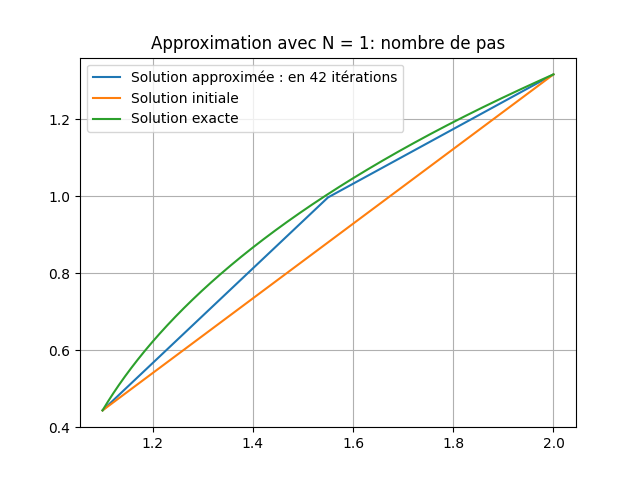
\includegraphics[width=0.75\linewidth]{approxWith1.png}
        \caption{Approximation avec N = 1}
        \label{fig:approx_N1}
    \end{figure}

    \begin{figure}[H]
        \centering
        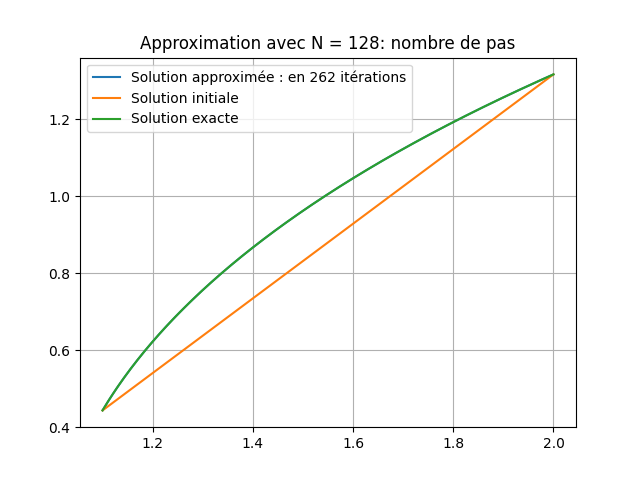
\includegraphics[width=0.75\linewidth]{approxWith128.png}
        \caption{Approximation avec N = 128}
        \label{fig:approx_N128}
    \end{figure}

    \textbf{Remarque :} Avec le code utilisé, $n$ est déterminé une fois que l'erreur est suffisamment petite, ce qui dépend de notre tolérance.
}

% question 7
\QuestionAnswer{
    On prend $\alpha = 0$, $a = 1$ et $\beta = \text{argch}(b)$. Montrer que la fonction $u_{\text{ex}} : r \in [a, b] \to \text{argch}(r)$ est bien solution du problème de minimisation de $\mathcal{J}$ sur $\SetC$.
}{
    On travaille sur l'ensemble :

    $$\SetC_\text{test} := \Set{v \in \Sobolev{[1, b]} : v(1) = 0, \, v(b) = argch(b) }$$

    On veut montrer que $d\FunctionJ(u_{\text{ex}})(\varphi) = 0 \quad \forall \varphi \in W^{1,1}_0[a,b]$

    C'est à dire :
    $$\Integral{a}{b}{ r \frac{u_{\text{ex}}'(r)\varphi'(r)}{\FunctionWithSqrt{u_{\text{ex}}'(r)}} }{r} = 0$$

    On calcule $u_{\text{ex}}'$ :

    $$u_{\text{ex}}'(x) = \frac{1}{\sqrt{x^2-1}}$$

    Soit $\varphi \in W^{1,1}_0[a,b]$
    \begin{align*}
        d\FunctionJ(u_{\text{ex}})(\varphi) &= \Integral{a}{b}{ r \frac{u_{\text{ex}}'(r)\varphi'(r)}{\FunctionWithSqrt{u_{\text{ex}}'(r)}} }{r} \\
        &= \Integral{a}{b}{ \frac{r \varphi'(r)}{\sqrt{r^2-1} \FunctionWithSqrt{\frac{1}{\sqrt{r^2-1}}}} }{r} \\
        &= \Integral{a}{b}{ \frac{ r \varphi'(r)}{
        \sqrt{r^2 - 1 + 1} }}{r} \\
        &= \Integral{a}{b}{ \varphi'(r) }{r} \\
        &= \varphi(b) - \varphi(a) \\
        &= 0 \quad \text{car } \varphi(a) = 0 \text{ et } \varphi(b) = 0 \\
    \end{align*}

    Donc $u_{\text{ex}}$ est bien solution du problème.
}

% question 8
\QuestionAnswer{
    Étudier l'erreur en fonction de $h$ en norme $L^1$ et en norme $W^{1,1}$ entre $u^n_h$ et $u_{\text{ex}}$ pour $n$ fixé assez grand. Que semble être l'ordre de la méthode en $h$?
}{
    Avec les mêmes paramètres qu'à la question 2.0.6 :
    
    \begin{figure}[H]
        \centering
        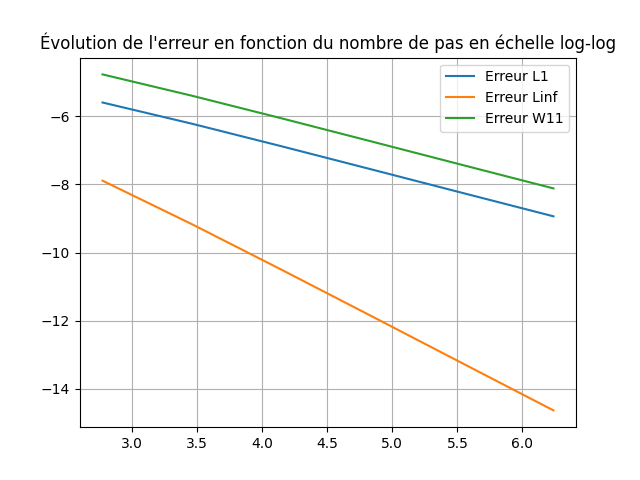
\includegraphics[width=0.75\linewidth]{errorsWith128.png}
        \caption{Erreurs avec N = 16, 32, ..., 512}
        \label{fig:errors_N128}
    \end{figure}

    \textbf{Remarque :} On a décidé de prendre en abscisse le nombre de pas, plutôt que $h$ la finesse. Mais c'est en réalité équivalent puisque le nombre de pas est inversement proportionnel à la finesse du maillage. Donc en échelle logarithmique, cela ne change que le signe.

    \textbf{Résultats du modèle :}
    \begin{itemize}
        \item Pente de l'erreur $L^1$:   0.9862943239012876
        \item Pente de l'erreur $L^{\infty}$: 1.9856410345335198
        \item Pente de l'erreur $W^{1,1}$:  0.9873503213327378
    \end{itemize}

    L'ordre de la méthode semble être $1$ avec les normes $L^1$ et $W^{1,1}$.

    \textbf{Remarque :} En norme $L^{\infty}$, on obtient l'ordre 2.
}

% question 9
\QuestionAnswer{
    Pour $n$ fixé assez grand, tracer la surface pour différentes valeurs de $h$, $\mathcal{S}_h = \Set{(x, y, u^n_h(x, y)) : (x, y) \in \Omega}$.
}{
    \begin{figure}[H]
        \centering
        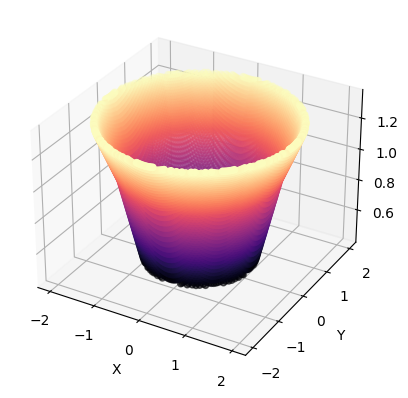
\includegraphics[width=0.75\linewidth]{surfaceWith1.png}
        \caption{Surface approximée avec N = 1}
        \label{fig:surface_N1}
    \end{figure}

    \begin{figure}[H]
        \centering
        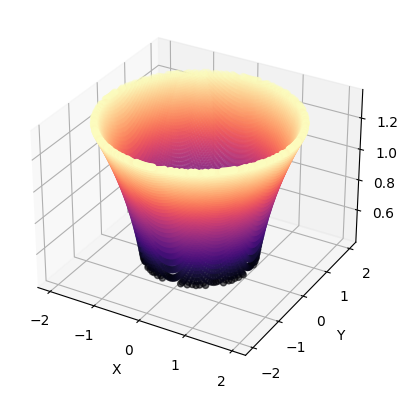
\includegraphics[width=0.75\linewidth]{surfaceWith32.png}
        \caption{Surface approximée avec N = 32}
        \label{fig:surface_N32}
    \end{figure}

    \begin{figure}[H]
        \centering
        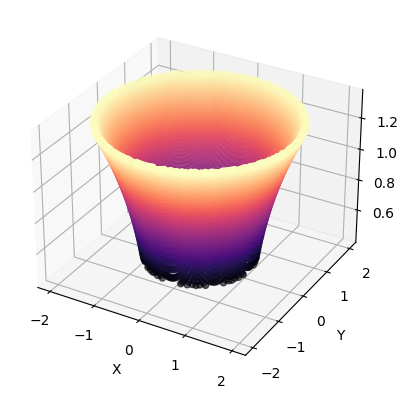
\includegraphics[width=0.75\linewidth]{surfaceWith128.png}
        \caption{Surface approximée avec N = 128}
        \label{fig:surface_N128}
    \end{figure}

    Pour $N=1$, on peut observer que la surface est composée de deux sections de cônes. Ce qui fait que pour $N = 32$ et $N = 128$, la surface est beaucoup plus lisse et il est difficile de visualiser de grandes différences avec une simple observation. On peut toutefois comparer avec la surface de la solution exacte et valider notre modèle :

    \begin{figure}[H]
        \centering
        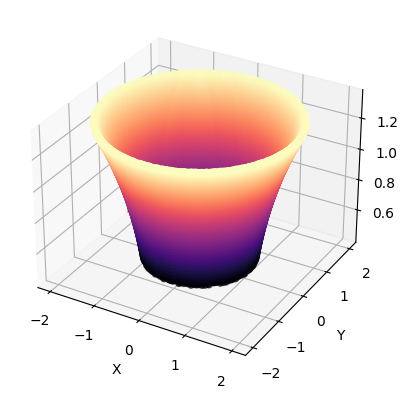
\includegraphics[width=0.75\linewidth]{surfaceWithExact.png}
        \caption{Surface de la solution exacte}
        \label{fig:surface_exact}
    \end{figure}

    Visuellement, le modèle semble bien se rapprocher de la solution, et les erreurs obtenues en question 2.0.8 tendent à le confirmer.
}

% = = = = = = = = = = = = = = = = = = = = = = = = = = = = = = = = =
\end{document}
